% !TeX root = Project.tex
\section{The Motivation}

Our goal when we integrate a function is to find the amount of `space' between the graph and x-axis (or the Abscissa if you're fancy --- but I'll just say x-axis). It's pretty difficult to say how much space an arbitrary curve takes up, but we can work out the area of rectangles very easily --- by calculating the {\em base $\times$ height}. Riemann integration takes advantage of this, and defines the integral of a function $f:\R \rightarrow \R$ by first bounding it from above with rectangular functions and finding the smallest of these areas (which is would be an upper bound for the area of the function), then we bound the function from below and find an lower bound, then we hope that these two bounds match up. 

\begin{figure}[H]
\centering
\begin{minipage}{.5\textwidth}
  \centering
  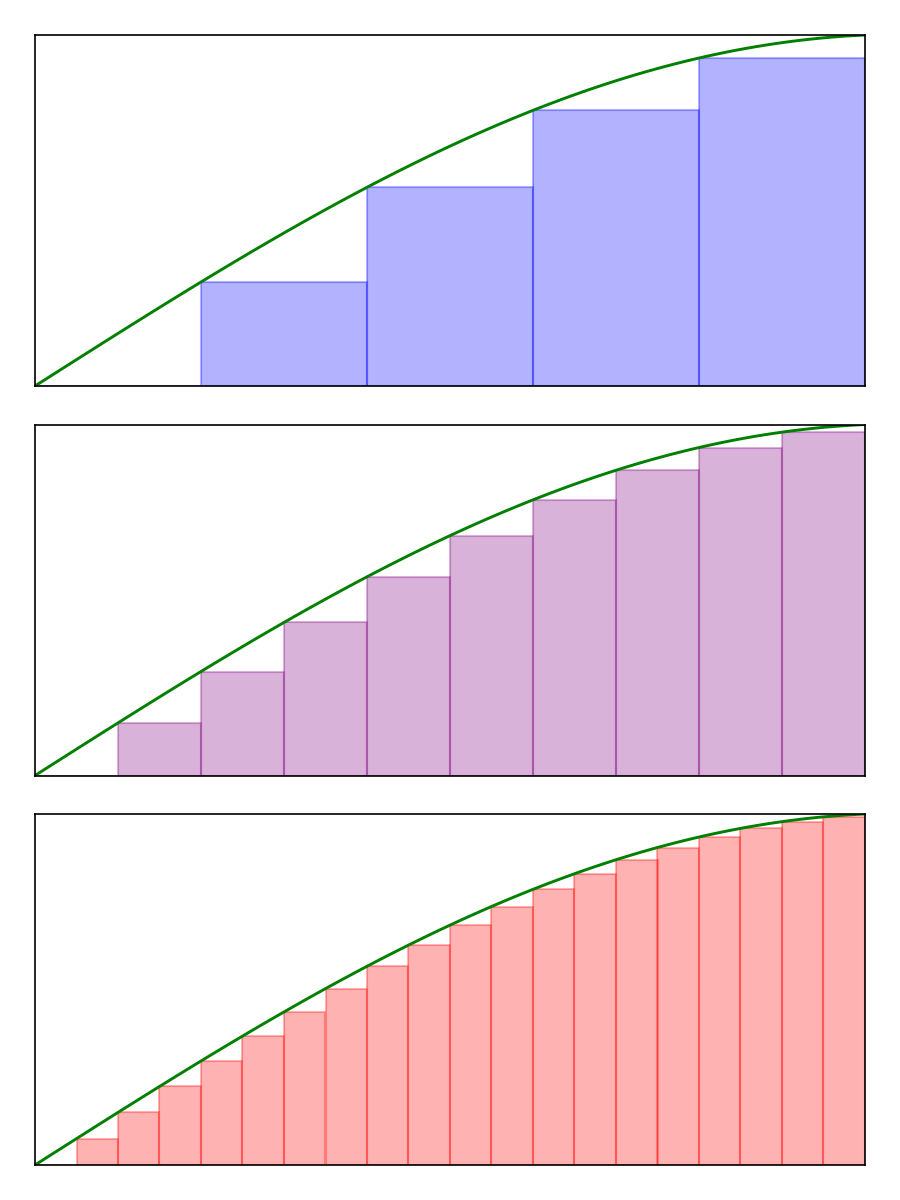
\includegraphics{Code/Area1.png}
  \captionof{figure}{Bounding from Below}
  \label{fig:areabelow}
\end{minipage}%
\begin{minipage}{.5\textwidth}
  \centering
  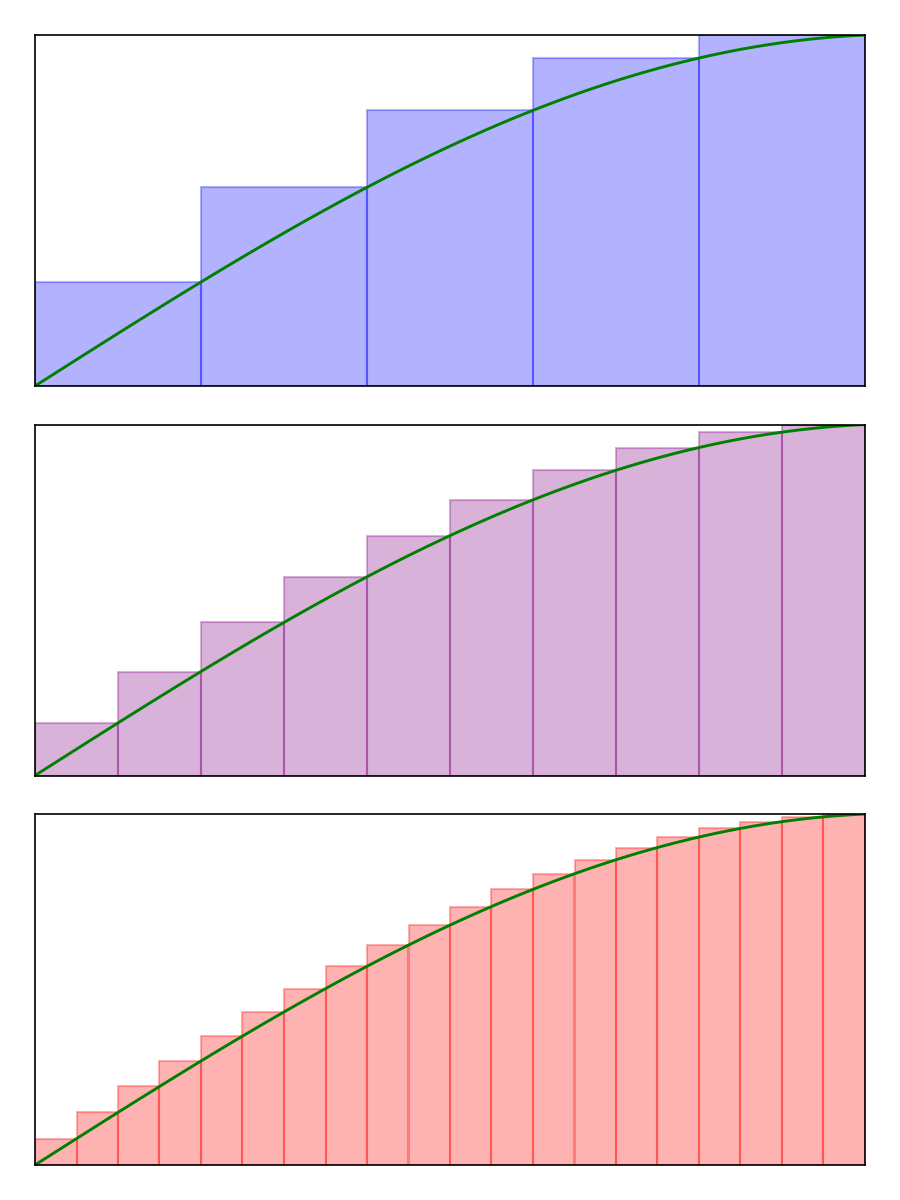
\includegraphics{Code/Area2.png}
  \captionof{figure}{Bounding from Above}
  \label{fig:areaabove}
\end{minipage}
\end{figure}

If the domain of our function (the `x-axis'), is $\R^2$ instead of just $\R$, we'd actually calculating a volume by finding the `space' between the graph and the axis. Basic Riemann integration doesn't apply to these functions --- still, you can think of the `area of a rectangle' (which in $R^2 \rightarrow \R$ would actually be the volume of a cuboid) as being calculated in much the same way; the size of the base (which is now an area, instead of a length) $\times$ the height. With this is mind, lets clear up some of the terms we are going to use:

\begin{description}
\item[\em Lebesgue integration\/] is the method of integration defined above. Just like Riemann Integration, it is used to find the space between the graph of a function and the domain. However, unlike Riemann, the domain can be any set at all. Thinking back to rectangles and cuboids and $base \times height$, if we wanted make sense of what it means for there to be space between the graph and the x-axis, we should be able to make sense of the `size' of parts of the domain, so that we can figure out how big our base is and multiply that by the height$\ldots$
%
\item[\em The Lebesgue Measure\/] seems then like it'd be a way to assign sizes to, or `measure' sets in the domain; but it is not! It's a term used specifically when we give sizes to the subsets of $\R^n$, and those sizes (or `measures') coincided with our usual idea of the size of a set in $\R^n$ --- i.e. it is used when we are considering functions $\R^n \supset Y \rightarrow \R$, and in $\R$ the measure (length) of the interval $[1, 0]$ is 1, in $\R^2$ the measure (area) of the rectangle $[1, 0] \times [1, 0]$ is 1, in $\R^3$ the measure (volume) of the cube $[1, 0] \times [1, 0] \times [1, 0]$ is 1$\ldots$ etc. 
%
\item[\bf \em The Lebesgue Integral\/] is what we get when we do Lebesgue Integration on a set with the Lebesgue Measure on it. i.e. it's the integral of normal functions $\R^n \supset Y \rightarrow \R$. This is the (basically) the same domain as the Riemann integral and so we'd want to check that the Lebesgue Integral and the Riemann integral match up --- and then see if the Lebesgue integral is better in some way.

To see the motivation behind the Lebesgue integral over Riemann, let's look at the canonical example of a function for which the Riemann integral fails; $f:\R \rightarrow \R,\ \ f(x) = \mathbbm{1}_\Q(x)$. This is also an example of a {\em Simple Function} since it is just the indicator function of a measurable set, but lets not get ahead of ourselves...
\end{description}
\begin{figure}[H]
	\centering
	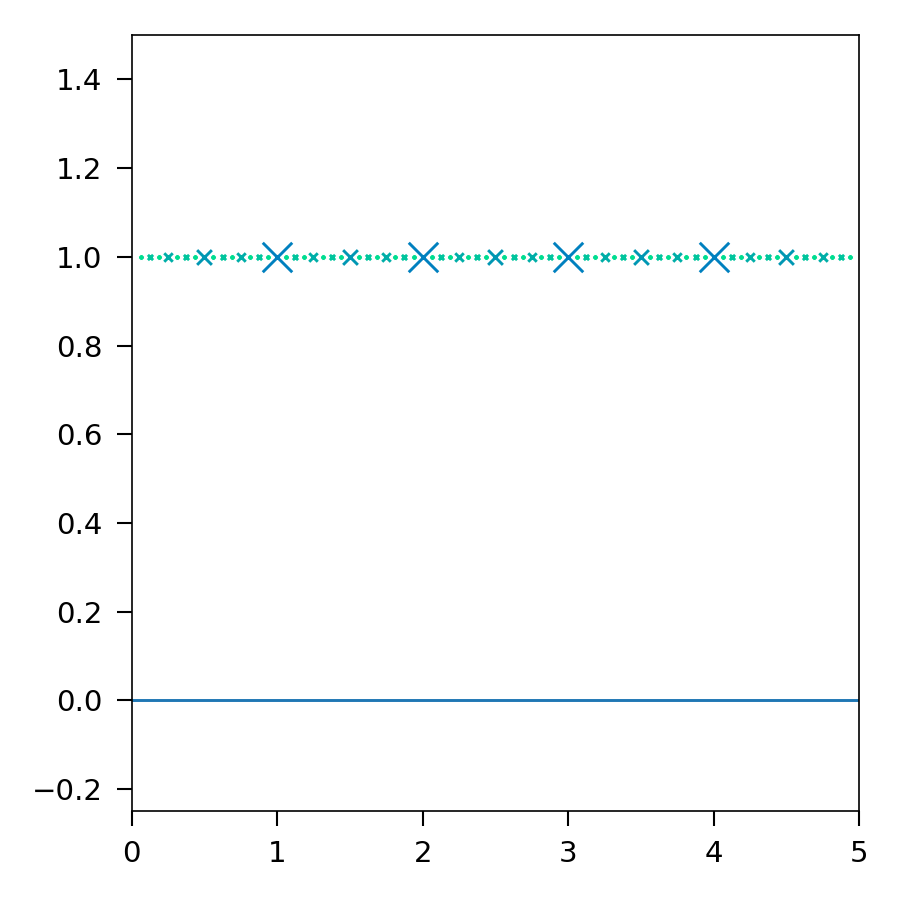
\includegraphics[]{Code/Rational.png}
	\caption{An illustration of the above indicator function, showing a few rationals that are multiples of negative powers of 2.}
\end{figure}

First, let's define the Riemann integral. The definition of the Riemann integral involves a few steps, and so it's going to take a little patience. The first step is defining a step function (no pun intended).
%
\begin{figure}[h]
	\centering
	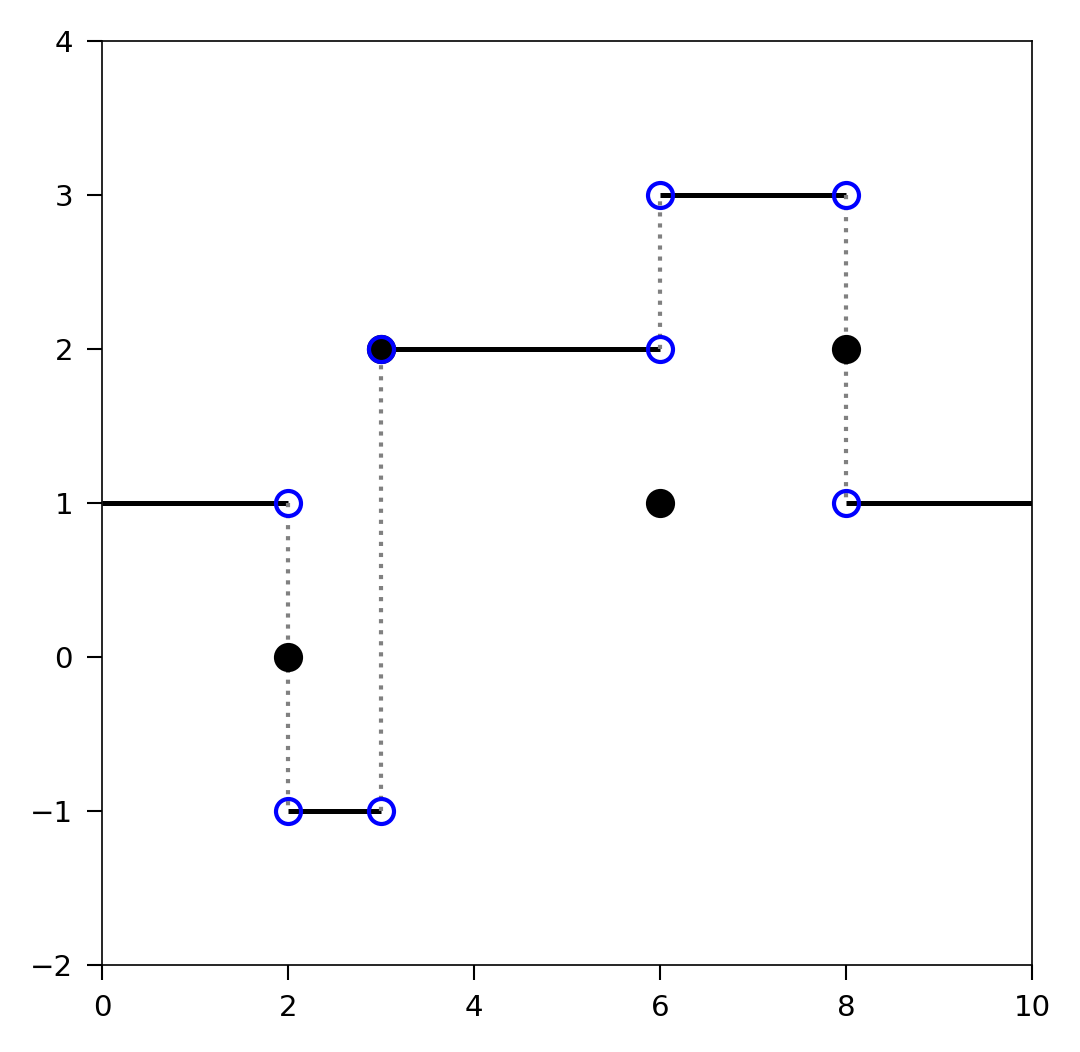
\includegraphics{Code/Step.png}
	\caption{A Step Function}
	\label{fig:step}
\end{figure}

A function is called a step function if and only if there exists some finite sequence of points (which we can index by n and call $x_n$) such that the function is constant between any two adjacent points. So for the function with the graph shown below in Figure \ref{fig:step}, the points $\{0, 2, 3, 6, 8, 10\}$ are the finite sequence which make this a step function. We can call sequence this a \emph{representation} of the function. 

Note two important points;
\begin{itemize}
	\item We could have picked $\{0, 1, 2, 3, 4, 5, 6, 7, 8, 9, 10\}$ to be our representation, since the function also happens to constant between any two adjacent integers. 
	\item It doesn't really matter what the function is {\em at} the points $x_n$ --- we only care whether the function is constant {\em between} the points. In our graph, 2, 3, 6, and 8 are discontinues, but that doesn't matter since they're also in our sequence of points. 
\end{itemize}

The formal definition is as follows;
\begin{definition}[\bf\em Step Function]
    $f\colon \ [a, b] \rightarrow \R$ is a {\em step function}
    \begin{itemize}
        \item[$\logeq$]
            $f \in \mathcal{S}([a, b])$
        \item[$\logeq$]
            $\exists N \! \in \! \N$ \ and \ $\exists X = (x_n)_{n=0}^N$ : $a = x_0 < x_1 < \ldots < x_{n-1} < x_n = b$, \ and \ $\forall m\in\N_{< N}$ we have $\exists! c_m \in \R$ : $\forall z \in (x_{m-1}, x_{m})$ we have $f(z) = c_m$.
    \end{itemize}
\end{definition}

This also defines \emph{the set of all step functions on} $[a, b]$ as $\mathcal{S}[a, b]$. This kind of thing is done a lot in analysis --- we often want to look at the set of all things which satisfy some property. We normally don't have to \emph{find} them all --- we just need a way to represent the full set. The fact that it'd be near impossible to try to imagine the set $\mathcal{S}([a, b])$ is irrelevant --- it's just important we know it exists.

Next, we want to define what it means to integrate a step function. Remember, the point of working with step functions is because it's easy to find the area of rectangles, and integration is all about finding areas. So where are the rectangles? 

As is hinted at by Figure \ref{fig:step}, we can make the bases of the rectangles the width the intervals $(x_{n-1}, x_n)$, and the heights the constant $c$ which values in this interval take. This is made even clearer by Figure \ref{fig:stepfilled}, where we can also see that the sometimes our heights will have negative values, and that's okay --- these areas are just taken away from the total area instead of added to it.
 
What's not okay is that any one step function may have different sequences which we can use to prove that it's a step function --- or in other words, the same step function may have different but equally valid representations. We defined the integral of a step function in terms it's representation, but how do we know that different representations of the same function produce the same integral? Figures \ref{fig:stepfilled} and \ref{fig:stepfilled10} demonstrate that, given the representations $\{0, 2, 3, 6, 8, 10\}$ and $\{0, 1, 2, \ldots, 10\}$ of \ref{fig:step}, we're fine, and the areas are equal. It turns out that this is the case in general --- the integral of a step function is independent of the chosen representation.

\begin{figure}[h]
\centering
\begin{minipage}{.5\textwidth}
  \centering
  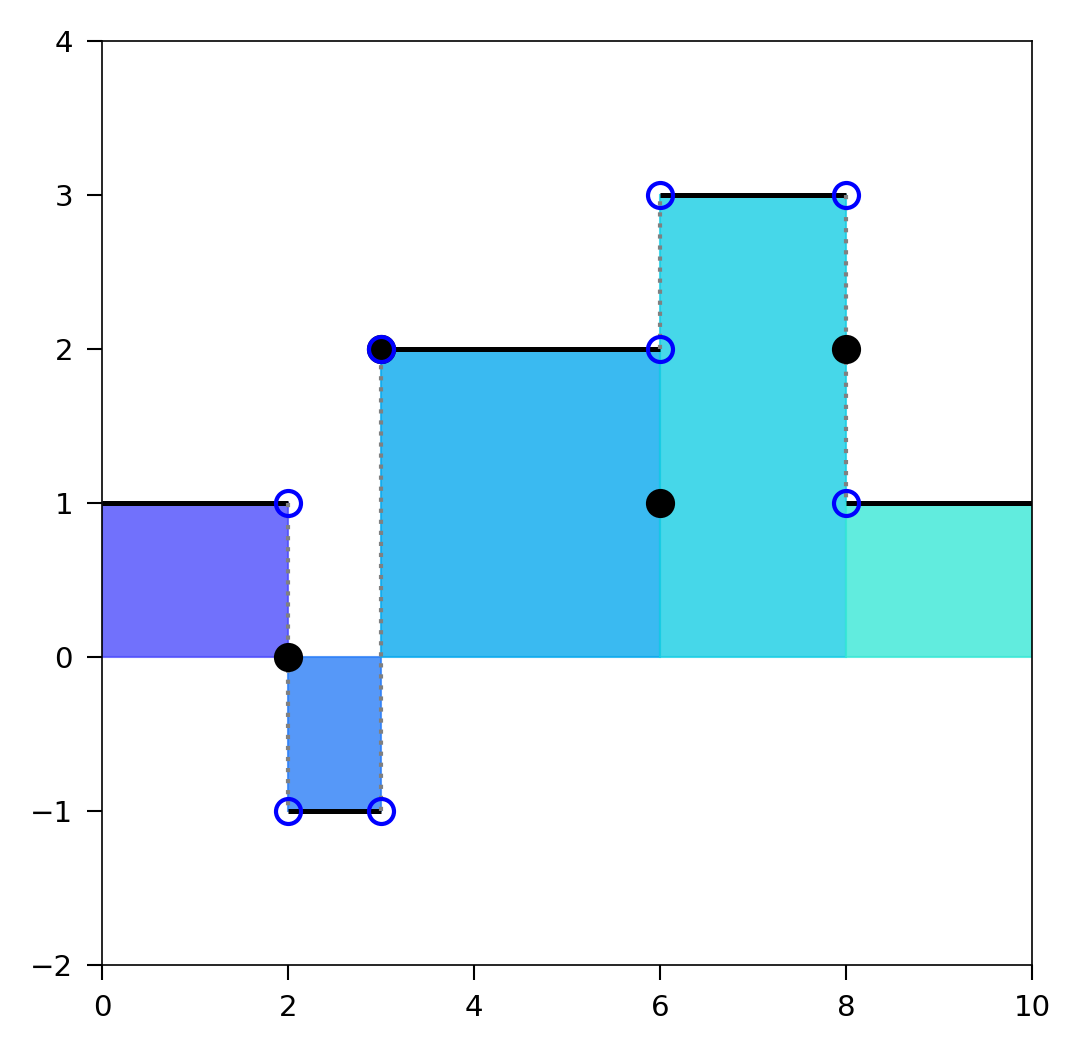
\includegraphics[scale=0.8]{Code/StepFilled3.png}
  \captionof{figure}{Integral of \ref{fig:step} using $\{0, 2, 3, 6, 8, 10\}$ }
  \label{fig:stepfilled}
\end{minipage}%
\begin{minipage}{.5\textwidth}
  \centering
  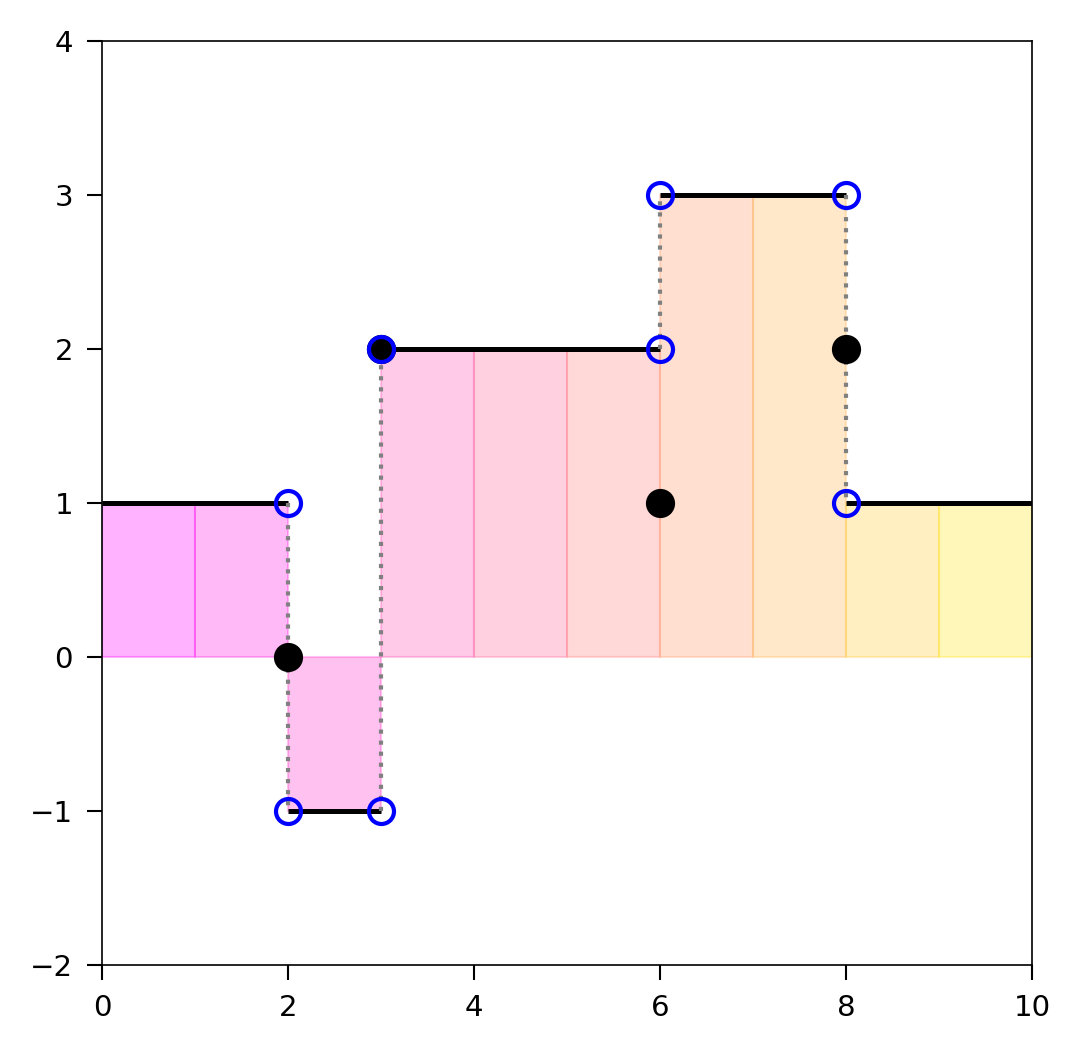
\includegraphics[scale=0.8]{Code/StepFilled.png}
  \captionof{figure}{Integral of \ref{fig:step} using $\{0, 1, 2, \ldots 10\}$}
  \label{fig:stepfilled10}
\end{minipage}
\end{figure}


